%%%%%%%%%%%%%%%%%%%%%%%%%%%%%%%%%%%%%%%%%
% Beamer Presentation
% LaTeX Template
% Version 1.0 (10/11/12)
%
% This template has been downloaded from:
% http://www.LaTeXTemplates.com
%
% License:
% CC BY-NC-SA 3.0 (http://creativecommons.org/licenses/by-nc-sa/3.0/)
%
%%%%%%%%%%%%%%%%%%%%%%%%%%%%%%%%%%%%%%%%%

%----------------------------------------------------------------------------------------
%	PACKAGES AND THEMES
%----------------------------------------------------------------------------------------

\documentclass{beamer}

\mode<presentation> {

% The Beamer class comes with a number of default slide themes
% which change the colors and layouts of slides. Below this is a list
% of all the themes, uncomment each in turn to see what they look like.

%\usetheme{default}
%\usetheme{AnnArbor}
%\usetheme{Antibes}
%\usetheme{Bergen}
%\usetheme{Berkeley}
%\usetheme{Berlin}
%\usetheme{Boadilla}
%\usetheme{CambridgeUS}
%\usetheme{Copenhagen}
%\usetheme{Darmstadt}
%\usetheme{Dresden}
%\usetheme{Frankfurt}
%\usetheme{Goettingen}
%\usetheme{Hannover}
%\usetheme{Ilmenau}
%\usetheme{JuanLesPins}
%\usetheme{Luebeck}
\usetheme{Madrid}
%\usetheme{Malmoe}
%\usetheme{Marburg}
%\usetheme{Montpellier}
%\usetheme{PaloAlto}
%\usetheme{Pittsburgh}
%\usetheme{Rochester}
%\usetheme{Singapore}
%\usetheme{Szeged}
%\usetheme{Warsaw}

% As well as themes, the Beamer class has a number of color themes
% for any slide theme. Uncomment each of these in turn to see how it
% changes the colors of your current slide theme.

%\usecolortheme{albatross}
%\usecolortheme{beaver}
%\usecolortheme{beetle}
%\usecolortheme{crane}
%\usecolortheme{dolphin}
%\usecolortheme{dove}
%\usecolortheme{fly}
%\usecolortheme{lily}
%\usecolortheme{orchid}
%\usecolortheme{rose}
%\usecolortheme{seagull}
%\usecolortheme{seahorse}
%\usecolortheme{whale}
%\usecolortheme{wolverine}

%\setbeamertemplate{footline} % To remove the footer line in all slides uncomment this line
%\setbeamertemplate{footline}[page number] % To replace the footer line in all slides with a simple slide count uncomment this line

%\setbeamertemplate{navigation symbols}{} % To remove the navigation symbols from the bottom of all slides uncomment this line
}

\usepackage{graphicx} % Allows including images
\usepackage{dirtytalk}
\usepackage{subfig}
\usepackage{booktabs} % Allows the use of \toprule, \midrule and \bottomrule in tables
% \usepackage[T1]{fontenc}
% \usepackage[font=small,labelfont=bf,tableposition=top]{caption}
\usepackage{multirow}

% \DeclareCaptionLabelFormat{andtable}{#1~#2  \&  \tablename~\thetable}

%----------------------------------------------------------------------------------------
%	TITLE PAGE
%----------------------------------------------------------------------------------------

\title[ROBUST PORTFOLIO OPTIMIZATION]{ROBUST PORTFOLIO OPTIMIZATION:\\
A STUDY OF BSE 30 AND BSE 100} % The short title appears at the bottom of every slide, the full title is only on the title page

\author{Mohammed Bilal Girach \\ Shashank Oberoi} % Your name
\institute[]{
Department of Mathematics \\ % Your institution for the title page
\medskip
%\textit{john@smith.com} % Your email address
IIT Guwahati
}
%\date{\today} % Date, can be changed to a custom date
\date{May 14, 2019}

\begin{document}

\begin{frame}
\titlepage % Print the title page as the first slide
\end{frame}

\begin{frame}
\frametitle{Outline} % Table of contents slide, comment this block out to remove it
\tableofcontents % Throughout your presentation, if you choose to use \section{} and \subsection{} commands, these will automatically be printed on this slide as an overview of your presentation
\end{frame}

%----------------------------------------------------------------------------------------
%	PRESENTATION SLIDES
%----------------------------------------------------------------------------------------

%------------------------------------------------
\section{Introduction to Robust Optimization} % Sections can be created in order to organize your presentation into discrete blocks, all sections and subsections are automatically printed in the table of contents as an overview of the talk
%------------------------------------------------

%\subsection{Subsection Example} % A subsection can be created just before a set of slides with a common theme to further break down your presentation into chunks

\begin{frame}{Introduction to Robust Optimization}{}
%\frametitle{Introduction}
\begin{itemize}
   \item{Emergence of Robust Optimization driven primarily by the necessity to address various demerits of Markowitz \cite{mark1} optimization such as}
   \begin{enumerate}
       \item Assigning extreme weights to the assets.
       \item High sensitivity of the optimal portfolio to the errors in estimates of input parameters.
   \end{enumerate}
   \item{Includes the class of methods proposed to optimize the portfolio performance using an \say{uncertainty set} that includes the worst possible realizations of the uncertain input parameters.}
   \item{Can be extended to the framework of risk minimization since there is an issue of lack of robustness with downside risk measures such as VaR and CVaR.}
   
    
\end{itemize}
\end{frame}

%------------------------------------------------



%------------------------------------------------
\section{Robust Portfolio Optimization Models}

\begin{frame}{Robust Portfolio Optimization Models}{Mathematical Formulations Using Uncertainty Sets}
\begin{itemize}
    \item {For any general uncertainty set $\displaystyle{\mathcal{U}_{\mu,\Sigma}}$, the worst case classical Markowitz model formulation with no short selling constraint is given as:
\begin{equation}
\label{eq:worst_case_classical_markowitz}
\max\limits_{\mathbf{x}}\left\{\min\limits_{\left(\boldsymbol{\mu},\boldsymbol{\Sigma}\right)~\in~\mathcal{U}_{\mu,\Sigma}}\boldsymbol{\mu}^{\top}\mathbf{x}
-\lambda\mathbf{x^{\top}}\Sigma\mathbf{x}\right\}~\text{such that}~\mathbf{x^{\top}}\mathbf{1}=1~\text{and}~\mathbf{x}~\geq 0,
\end{equation}}
   \item{ We mainly deal with three types of uncertainty sets, namely, box and ellipsoidal (for expected returns) and separable (for both expected returns and covariance matrix of returns).}
   \item{\textbf{Box Model}:
   Box uncertainty in terms of expected returns can be expressed as:
\begin{equation}
U_{\boldsymbol{\delta}}(\boldsymbol{\hat{\mu}}) = \left\{ \boldsymbol{\mu}: | \mu_i - \hat{\mu_i}| \leq \delta_i, i = 1,2,3,...,N \right\}    
\end{equation}
Accordingly, we obtain the following robust formulation 
\begin{equation}
\label{eqn:trans_eqn_box}
\max_\mathbf{x} \quad \boldsymbol{\hat{\mu}}^{\top} \, \mathbf{x}-  \lambda \mathbf{x^{\top}}\Sigma \, \mathbf{x} - \boldsymbol{\delta}^{\top}|\mathbf{x}| \quad \text{such that } \mathbf{x^{\top}}\mathbf{1}  = 1 \text{ and } \mathbf{x} \geq 0,  
\end{equation}}
\end{itemize}
\end{frame}


\begin{frame}{Robust Portfolio Optimization Models}{Mathematical Formulations Using Uncertainty Sets}
\begin{itemize}
\item{\textbf{Ellip Model}:
   Ellipsoidal uncertainty set for expected return $\left(\boldsymbol{\mu}\right)$ is:
\begin{equation}
\label{eqn:ellipsoidal}
U_{\delta}(\boldsymbol{\hat{\mu}})=\left\{\boldsymbol{\mu}: (\boldsymbol{\mu}-\boldsymbol{\hat{\mu}})^{\top}\Sigma^{-1}_{\boldsymbol{\mu}}
(\boldsymbol{\mu}-\boldsymbol{\hat{\mu}})\leq\delta^2 \right\}.
\end{equation}
Using ellipsoidal set, the following robust optimization is obtained
\begin{equation}
\label{eqn:ellipsoidal_markowitz}
\max\limits_{\mathbf{x}}\left\{\boldsymbol{\hat{\mu}}^{\top}\mathbf{x}-\lambda \mathbf{x}^{\top}\Sigma_{\boldsymbol{\mu}}\mathbf{x}
-\delta\sqrt{\mathbf{x}^{\top}\Sigma_{\boldsymbol{\mu}}\mathbf{x}}\right\}~\text{such that}~\mathbf{x^{\top}}\mathbf{1}=1~\text{and}~\mathbf{x}\geq 0.
\end{equation}
   }
   \item{\textbf{Sep Model}: Separable uncertainty set  is given as:
   \begin{equation}
\label{eqn:separable}
\begin{split}
& U_{\Sigma}=\{\Sigma: \underline{\Sigma} \leq \Sigma \leq \overline{\Sigma},~\Sigma \succeq 0\} \\
& U_{\boldsymbol{\mu}}=\{\boldsymbol{\mu}:\underline{\boldsymbol{\mu}}\leq\boldsymbol{\mu}\leq\overline{\boldsymbol{\mu}}\},
\end{split}
\end{equation}
Consequently, we obtain the following robust formulation:
\begin{equation}
\label{eqn:separable_markowitz}
\max_{\mathbf{x}} \left\{\underline{\boldsymbol{\mu}}^{\top}\mathbf{x}-\lambda \mathbf{x^{\top}}\overline{\Sigma}\mathbf{x}\right\}~\text{such that}~ \mathbf{x^{\top}}\mathbf{1}=1~\text{and}~\mathbf{x}\geq 0.
\end{equation}}
\end{itemize}
\end{frame}



\begin{frame}{Robust Portfolio Optimization Models}{Computational Results}
\begin{itemize}
    \item{Analysis performed under two scenarios:
    \begin{enumerate}
        \item{Number of stocks $N=31$}
        \item{Number of stocks $N=98$}
    \end{enumerate}
    }
    \item{For each scenario, following data used:
    \begin{enumerate}
        \item{Log-returns based on daily Adjusted Close Price of stocks comprising BSE30 for Scenario 1 and BSE100 for Scenario 2 (Yahoo Finance).}
        \item{Simulated Data with $\#$samples for returns same as in market data, say $\zeta (<1000)$.}
        \item{Simulated Data with $\#$samples$=1000$.}
    \end{enumerate}
    }
    \item{Sharpe Ratio used as performance measure for comparing robust models with Markowitz Model (Mark) with annualized risk-free rate assumed equal to $6\%$.}
    \item{Portfolio optimization within ideal range of risk-aversion ($\lambda \in [2,4]$). }
    \item{Uncertainty sets constructed with $95\%$ confidence level. }
\end{itemize}
\end{frame}

\begin{frame}{Robust Portfolio Optimization Models}{Computational Results}

\begin{itemize}
    \item{Performance with $N=31$ assets:
    \begin{block}{Common observation inferred from three cases}
Sep and Ellip model perform superior or equivalent in comparison to Markowitz model in the ideal range of risk-aversion.
\end{block}
    }
    \item{Performance with $N=98$ assets:
    \begin{block}{Common observation inferred from three cases}
Sep and Ellip model outperform the Markowitz model in the ideal range of risk-aversion.
\end{block}
    }
\end{itemize}

\end{frame}

\section{VaR and Its Robust Formulation}

\begin{frame}{VaR and Its Robust Formulation}{Introduction}
In the preceding chapters, we observed several limitations of the mean-variance framework such as:
\begin{itemize}
    \item Sensitivity to errors in data as well as in the
estimation of mean and variance of the underlying distribution.
    \item The use of standard deviation as a measure of risk as it takes both upside and downside risks into account.
    \item Variance is not a reliable or appropriate risk measure, if the underlying distribution is leptokurtic.
\end{itemize}

In order to address these issues, Value at Risk (VaR) which takes probability of losses (downside risk) into account became the popular choice.
% With asymmetric distributions, though, there can be a difference between upside and downside risk. As we noted  in  chapter  3,  studies  of  risk  aversion in  humans  conclude  that  (a)  they  are  loss averse, i.e., they weigh the pain of a loss more than the joy of an equivalent gain and (b) they value very large positive payoffs – long shots – far more than they should given the likelihood of these payoffs

%  Return distributions   for   stocks and most   other   assets are   not symmetric and exhibit fat tails. Critics of the mean variance approach argue that it takes too narrow a view of both rewards and risk.  In  their  view,  a  fuller  return  measure  should  consider  not  just  the  magnitude  of expected returns but also the likelihood of very large positive returns or skewness and more  complete  risk  measure  should  incorporate  both  variance  and possibility  of  big jumps (co-kurtosis).
\end{frame}

\begin{frame}{VaR and Its Robust Formulation}{Introduction}
However, VaR has its own limitations:
\begin{itemize}
    \item For the computation part, it requires the knowledge of the whole distribution.
    \item The computation also involves high dimensional numerical integration which may not be tractable at times.
    \item Black and Litterman \cite{black}, Pearson and Ju \cite{ju98} determined that the error in the computation of the VaR can be attributed to errors in the estimation of the first and second moments of the asset returns.
\end{itemize}
With the emergence of the robust formulations and optimizations, the concept of worst-case VaR (WVaR) not only allows for approaching the solution in a more tractable way, but also relaxes the assumptions on the information known to us apriori.

% Here, we assume that only partial information about the underlying distribution is known. We also assume that the distribution of the asset returns belong to a family of allowable probability distributions $\mathcal{P}$

\end{frame}
\begin{frame}{VaR and Its Robust Formulation}{Mathematical Formulation for Base-Case VaR model}
Ghaoui et al. defined VaR as the minimum value
of $\gamma$ such that the probability of loss exceeding $\gamma$ is less than $\epsilon$
\begin{equation}
\begin{split}
VaR_\epsilon(\mathbf{x}) = \min \, \left\{ \gamma :  \, P\left\{\gamma \leq -r(\mathbf{x},\boldsymbol{\mu})\right\} \leq \epsilon \right\}, \text{where } \epsilon \in (0,1), \\
\end{split}
\label{fig:var_basic}
\end{equation}

In the VaR framework, the knowledge of the entire distribution is necessary for the computation part. If the underlying distribution is Gaussian with the moments' pair as ($\hat{\boldsymbol{\mu}}$, $\Sigma$), then VaR can be computed via the following analytical form:
\begin{equation}
\begin{split}
VaR_\epsilon(\mathbf{x}) = \kappa(\epsilon)\sqrt{\mathbf{x}^{\top}\Sigma \mathbf{x}} - \hat{\boldsymbol{\mu}}^{\top}\mathbf{x}, \, \text{  where} \kappa(\epsilon) = -\Phi^{-1}(\epsilon),
\end{split}
\label{eqn:kappa_eqn}
\end{equation}
However, if the distribution is unknown, we use the bound given by Bertsimas and Popescu \cite{bertsimas05} \textit{i.e.,} $\displaystyle{ \kappa(\epsilon) = \sqrt{\frac{1-\epsilon}{\epsilon}}}$. Finally, we formulate the generalised VaR as follows:
\begin{equation}
\begin{split}
VaR_\epsilon(\mathbf{x}_{opt}) = \min \, \kappa(\epsilon)\sqrt{\mathbf{x}^{\top}\Sigma \mathbf{x}} - \hat{\boldsymbol{\mu}}^{\top}\mathbf{x} \quad \text{subject to } \quad \mathbf{x} \in \mathcal{X},
\end{split}
\label{fig:var_general}
\end{equation}
\end{frame}


\begin{frame}{VaR and Its Robust Formulation}{Mathematical Formulation for Worst-Case VaR model}
Here, we assume that only partial information about the
underlying distribution is known. We also assume that the distribution of the asset returns belong to a family of allowable probability distributions $\mathcal{P}.$

Given a probability level $\epsilon$, the worst-case VaR can be formulated as 
\begin{equation}
\begin{split}
VaR_{\epsilon}^{\mathcal{P}}(\mathbf{x}) = \min \, \left\{\gamma : \, \sup_{P \in \mathcal{P}} P\left\{\gamma \leq -r(\mathbf{x},\boldsymbol{\mu})\right\} \leq \epsilon \right\},
\end{split}
\label{fig:wc_var_basic}
\end{equation}
and accordingly, the robust formulation can be written as 
\begin{equation}
\begin{split}
WVaR_\epsilon(\mathbf{x}_{opt}) = \min \, VaR_{\epsilon}^{\mathcal{P}}(\mathbf{x}) \quad \text{subject to} \quad \mathbf{x} \in \mathcal{X}, 
\end{split}
\label{fig:wc_var_general}
\end{equation}

Using the notion of separable uncertainty sets, (\ref{fig:wc_var_general}) transforms to the following optimization problem:
\begin{equation}
\begin{split}
\min \, \kappa(\epsilon)\sqrt{\mathbf{x}^{\top}\overline{\Sigma}\mathbf{x}} - \underline{\hat{\boldsymbol{\mu}}}^{\top}\mathbf{x} \quad \text{subject to } \quad \mathbf{x} \in \mathcal{X},
\end{split}
\label{fig:var_poly}
\end{equation}
\end{frame}
\begin{frame}{VaR and Its Robust Formulation}{Computational Results: Implementation details}
\begin{itemize}
    \item We carry out the analysis in a similar fashion as we have completed for mean-variance setup. On the same lines, we use Sharpe Ratio (SR) as a metric to compare the performance of the portfolios where the  annualised risk-free rate is taken as 6\%.
    \item We perform the empirical analysis for the available historical data for S\&P BSE 30 (N = 31) and S\&P BSE 100 (N = 98). In each environment, we use additional two sets of simulated data with varying number of simulations.
    \item We only consider the values of $\epsilon$ to be in (0,0.1) i.e., the confidence level is greater than or equal to 90\%.
\end{itemize}
\end{frame}

\begin{frame}{VaR and Its Robust Formulation}{Computational Results: Performance with $N=31$ and $N=98$ assets}
\begin{table}[!h]
\centering
\tiny
\captionsetup{justification=centering}
\begin{tabular}{||c|c|c|c|c|c|c||}
\hline
$\epsilon$ & $\mu_{VaR}$ & $\sigma_{VaR}$ & $\mu_{WVaR}$ & $\sigma_{WVaR}$ & $SR_{VaR}$ & $SR_{WVaR}$\\
\hline
0.0001 & 0.000646 & 0.00522 & 0.000603 & 0.00528 & 0.0932 & 0.0839 \\
0.0201 & 0.000715 & 0.00522 & 0.00066 & 0.00529 & 0.106 & 0.0947 \\
0.0401 & 0.000744 & 0.00523 & 0.000687 & 0.0053 & 0.112 & 0.0995 \\
0.0601 & 0.000763 & 0.00523 & 0.000708 & 0.0053 & 0.115 & 0.103 \\
0.0801 & 0.000777 &0.00524 & 0.000726 & 0.00531 & 0.118 & 0.107 \\
\hline
& & & & Avg & 0.111	& 0.0998 \\
\hline
\end{tabular}
\caption{Empirical Analysis of Base VaR and WVaR models in case of Market Data (31 assets)}
\label{tab:5.1}
\end{table}

\begin{table}[!h]
\centering
\tiny
\captionsetup{justification=centering}
\begin{tabular}{||c|c|c|c|c|c|c||}
\hline
$\epsilon$ & $\mu_{VaR}$ & $\sigma_{VaR}$ & $\mu_{WVaR}$ & $\sigma_{WVaR}$ & $SR_{VaR}$ & $SR_{WVaR}$\\
\hline
0.0001 & 0.000667 & 0.00484 & 0.00071 & 0.00496 & 0.105 & 0.111 \\ 
0.0201 & 0.000713 & 0.00485 & 0.000755 & 0.00497 & 0.114 & 0.12 \\
0.0401 & 0.000735 & 0.00485 & 0.000776 & 0.00498 & 0.119 & 0.124 \\
0.0601 & 0.000751 & 0.00486 & 0.000793 & 0.00499 & 0.122 & 0.127 \\
0.0801 & 0.000765 & 0.00486 & 0.000807 & 0.005 & 0.124 & 0.13 \\
\hline
& & & & Avg & 0.119 & 0.124 \\
\hline
\end{tabular}
\caption{Empirical Analysis of Base VaR and WVaR models in case of market data (98 assets)}
\label{tab:5.4}
\end{table}
\end{frame}

\begin{frame}{VaR and Its Robust Formulation}{Computational Results: Performance with $N=31$ and $N=98$ assets}
\begin{figure}[!h]
\centering
\includegraphics[height=3.825cm,width=0.35\textwidth]{VaR/bse30_market/sr_cheb.eps}
\caption{Sharpe ratio plot for Base VaR and WVaR models in case of Market data (31 assets)}
\label{fig:5.1}
\end{figure}

\begin{block}{Common inferences from three cases for $N=31$}
We observe that the Base case VaR model outperforms or performs at par with the WVaR model irrespective of the data type.
\end{block}
\end{frame}

\begin{frame}{VaR and Its Robust Formulation}{Computational Results: Performance with $N=31$ and $N=98$ assets}
\begin{figure}[!h]
\centering
\includegraphics[height=3.825cm,width=0.35\textwidth]{VaR/bse100_market/sr_cheb.eps}
\caption{Sharpe ratio plot for Base VaR and WVaR models in case of Market data (98 assets)}
\label{fig:5.4}
\end{figure}

\begin{block}{Common inferences from three cases for $N=98$}
We observe that the Worst case VaR (WVaR) model outperforms the base case VaR model irrespective of the data type.
\end{block}

\end{frame}

\section{CVaR and Its Robust Formulation}

\begin{frame}{CVaR and Its Robust Formulation}{Introduction}

\begin{itemize}
    \item{Conditional Value-at-Risk (CVaR), introduced by Rockafellar and Uryasev \cite{rockafellar1}, is defined as the expected loss conditioned on the loss outcomes exceeding VaR for continuous distributions.}
    \item{ CVaR has emerged as a viable risk measure and has addressed various concerns centred around VaR such as:
    \begin{enumerate}
        \item Lack of sub-additivity
        \item Lack of information on the size of losses in adverse scenarios \textit{i.e,} those beyond the confidence level ($1-\epsilon$)
        \item Non-convex nature of the optimization problem.
    \end{enumerate}
    }
    \item{Since computing CVaR requires the complete knowledge of the return distribution, it led to the introduction of a robust risk measure, namely, Worst-Case CVaR (WCVaR), by Zhu and Fukushima \cite{zhu}.}
    \item{Both CVaR and WCVaR are coherent measures of risk.}
\end{itemize}

\end{frame}



\begin{frame}{CVaR and Its Robust Formulation}{Mathematical Formulation for Base-Case CVaR model}
\begin{itemize}
    \item{ For $\epsilon \in (0,1)$ , CVaR, at confidence level $1-\epsilon$, is defined as:
\begin{equation}
\label{eq:6.1}
CVaR_{\epsilon}(\mathbf{x}) \triangleq \frac{1}{\epsilon} \, \int \limits_{-\mathbf{r}^{\top}\mathbf{x} \geq VaR_{\epsilon}(\mathbf{x})} p(\mathbf{r})  d\mathbf{r}
\end{equation}
where $\mathbf{r}$ is the random return vector having probability density function $p(\mathbf{r})$ and $\mathbf{x}$ is the weight vector for a portfolio.}

\item{As proved by Rockafeller and Uryasev \cite{rockafellar1}, $CVaR_{\epsilon}(\mathbf{x})$, defined in equation (\ref{eq:6.1}), can be transformed into: 
\begin{equation}
\label{eq:6.4}
CVaR_{\epsilon}(\mathbf{x}) = \min_{\gamma \in \mathcal{R}^{n}} F_{\epsilon}(\mathbf{x},\gamma)
\end{equation}
where $n$ is number of assets in the portfolio and $F_{\epsilon}(\mathbf{x},\gamma)$ is defined as:
\begin{equation}
\label{eq:6.5}
 F_{\epsilon}(\mathbf{x},\gamma) \triangleq \gamma \, + \, \frac{1}{\epsilon} \, \int \limits_{\mathbf{r} \in \mathcal{R}^{n}} [-\mathbf{r}^{\top}\mathbf{x}-\gamma]^{+} p(\mathbf{r})  d\mathbf{r}
\end{equation} }
\end{itemize}
\end{frame}

\begin{frame}{CVaR and Its Robust Formulation}{Mathematical Formulation for Base-Case CVaR model}
\begin{itemize}
\item{The problem of approximation of the integral involved in the equation (\ref{eq:6.5}) can be dealt by sampling the probability distribution of $\mathbf{r}$ as per its density $p(\mathbf{r})$, assuming $S$ samples $\{ \mathbf{r}_{1}, \mathbf{r}_{2}, .., \mathbf{r}_{i},..,\mathbf{r}_{S}\}$ for the return vector $\mathbf{r}$. In accordance with above approximation, the problem of minimization of classical CVaR, assuming no short-selling constraints, can be formulated as the following LLP:
\begin{equation}
\label{eq:6.7}
\begin{split}
& \min_{(\mathbf{x},\mathbf{u},\gamma,\theta)} \, \theta \, \, s.t. \\
& \mathbf{x}^{\top}\mathbf{1}=1, \mathbf{x} \geq \mathbf{0}, \\
& \gamma \, + \, \frac{1}{S \, \epsilon} \mathbf{1}^{\top}\mathbf{u} \leq \theta, \\
& u_{i} \geq -\mathbf{r}_{i}^{\top}\mathbf{x}-\gamma, \, u_{i} \geq 0, \, i=1,2,..,S. \\
\end{split}
\end{equation}
where the auxiliary vector $\mathbf{u} \in \mathcal{R}^S$ and $\theta$ is the auxiliary variable that is optimized to obtain the optimal value of the Base-Case CVaR.}
\end{itemize}
\end{frame}

\begin{frame}{CVaR and Its Robust Formulation}{Mathematical Formulation for Worst-Case CVaR model}
\begin{itemize}
    \item{At confidence level $1-\epsilon$, WCVaR is defined as:
\begin{equation}
\label{eq:6.2}
WCVaR_{\epsilon}(\mathbf{x}) \triangleq \sup_{p(\mathbf{r}) \in \mathcal{P}}CVaR_{\epsilon}(\mathbf{x})
\end{equation}
where $\mathcal{P}$ is some set of probability distributions.}
\item{Assuming that the return distribution belongs to a set of distributions comprising of all possible mixtures of some prior likelihood distributions, $WCVaR_{\epsilon}(\mathbf{x})$ can be rewritten as:
\begin{equation}
\label{eq:6.9}
\begin{split}
& WCVaR_{\epsilon}(\mathbf{x}) = \min_{\alpha \in \mathcal{R}} \max_{j \in \mathcal{L} } F_{\epsilon}^{j}(\mathbf{x},\gamma) \, , \, \text{where} \\
& \mathcal{L} \triangleq \{ 1,2,..,l \} \\
& F_{\epsilon}^{j}(\mathbf{x},\gamma) \triangleq \gamma \, + \, \frac{1}{\epsilon} \, \int \limits_{\mathbf{r} \in \mathcal{R}^{n}} [-\mathbf{r}^{\top}\mathbf{x}-\gamma]^{+} p^{j}(\mathbf{r})  d\mathbf{r} \\
\end{split}
\end{equation}
where $p^{j}(\mathbf{r})$ denotes the $j^{th}$ likelihood distribution and $l$ is the number of the likelihood distributions.}
\end{itemize}

\end{frame}

\begin{frame}{CVaR and Its Robust Formulation}{Mathematical Formulation for Worst-Case CVaR model}
\begin{itemize}
    \item{ 
    \begin{equation}
\label{eq:6.11}
\begin{split}
& \min_{(\mathbf{x},\mathbf{u},\gamma,\theta)} \, \theta \, \, s.t. \\
& \mathbf{x}^{\top}\mathbf{1}=1, \mathbf{x} \geq \mathbf{0}, \\
& \gamma \, + \, \frac{1}{S_{j} \, \epsilon} \mathbf{1}^{\top}\mathbf{u}^{j} \leq \theta, \, \, j=1,2,..,l,\\
& u_{i}^{j} \geq -\mathbf{r}_{i,j}^{\top}\mathbf{x}-\gamma, \, u_{i}^{j} \geq 0, \, \, i=1,2,..,S_{j}, \, \, j=1,2,..,l. \\
\end{split}
\end{equation}
In the above equation, $\mathbf{r}_{i,j}$ is the $i^{th}$ sample of the return with respect to $j^{th}$ likelihood distribution and $S_{j}$ is the number of samples corresponding to $j^{th}$ likelihood distribution. The auxiliary vector $\mathbf{u}=(\mathbf{u}^{1} ; \mathbf{u}^{2} ; .. ; \mathbf{u}^{l}) \in \mathcal{R}^{S}$ where $\displaystyle{S=\sum_{j=1}^{l}S_{j}}$ and $\theta$ is the auxiliary variable whose optimization yields the optimal value.}
\end{itemize}
\end{frame}

\begin{frame}{CVaR and Its Robust Formulation}{Computational Results : Implementation details}
\begin{itemize}
    \item{Similar to the robust methods in Markowitz optimization and VaR minimization, the empirical analysis of the Worst-Case CVaR  model vis-\`a-vis the Base-Case CVaR model is performed under two scenarios, namely, $N=31$ and $N=98$, using the same three sets of data.}
    \item{For computation of the Base-Case CVaR model, $S$ in equation (\ref{eq:6.7}) is set equal to the number of return samples, \textit{i.e,} either $\zeta$ or $1000$, depending upon the set of data used.}
    \item{Computation of the Worst-Case CVaR model is performed for values of $l$ in $\{2,3,4,5\}$ by setting $\displaystyle{S_{j}=\frac{S}{l}}$ where $\displaystyle{j \in \{1,2,..,l \}}$.}
    \item{Comparative study performed using the Sharpe Ratio of the constructed portfolios having confidence level greater than $90\%$, \textit{i.e,} $\epsilon \in (0,0.1)$.}
\end{itemize}
\end{frame}

\begin{frame}{CVaR and Its Robust Formulation}{Computational Results : Performance with $N=31$ assets}
\begin{table}[!h]
    \centering
    \small
    \captionsetup{justification=centering}

   \begin{tabular}{||c|c|c|c||}
   \hline
  
$l$ & $Avg. \, \, SR_{CVaR}$ & $Avg. \, \, SR_{WCVaR}$ & $Diff. \, \, in \, \, Avg. \, \, SR$ \\
  
  \hline
2 & 0.0856 & 0.0611 & -0.0245 \\
3 & 0.0856 & 0.0345 & -0.0511 \\
4 & 0.0856 & 0.0439 & -0.0417 \\
5 & 0.0856 & 0.031 & -0.0546 \\
  \hline
\end{tabular}
    \caption{Comparison of CVaR and WCVaR in case of Market Data for different values of $l$}
    \label{avgtab:6.1}
\end{table}

\begin{table}[!h]
    \centering
    \small
    \captionsetup{justification=centering}

   \begin{tabular}{||c|c|c|c|c|c|c||}
   \hline
  
$\epsilon$ & $\mu_{CVaR}$ & $\sigma_{CVaR}$ & $\mu_{WCVaR}$ & $\sigma_{WCVaR}$ & $SR_{CVaR}$ & $SR_{WCVaR}$\\
  
  \hline
0.0001 & 0.000266 & 0.00661 & 0.000266 & 0.00661 & 0.0162 & 0.0162 \\
0.0201 & 0.000545 & 0.00595 & 0.000266 & 0.00661 & 0.0648 & 0.0162 \\
0.0401 & 0.000706 & 0.00569 & 0.000514 & 0.00603 & 0.096 & 0.0587 \\
0.0601 & 0.000832 & 0.00557 & 0.000645 & 0.00598 & 0.121 & 0.0812 \\
0.0801 & 0.000877 & 0.00576 & 0.000696 & 0.00597 & 0.125 & 0.0897 \\
  \hline
\end{tabular}
    \caption{Empirical Analysis of CVaR and WCVaR in case of Market Data for $l=2$}
    \label{tab:6.1}
\end{table}


\end{frame}

\begin{frame}{CVaR and Its Robust Formulation}{Computational Results : Performance with $N=31$ assets}

\begin{figure}[!h]
    \centering
   
    \includegraphics[height=3.825cm,width=0.35\textwidth]{CVaR/bse30_market/sr_cvar_2.eps}

  \caption{Sharpe ratio plot for CVaR and WCVaR in case of Market Data for $l=2$}
  \label{fig:6.1}
\end{figure}

\begin{block}{Common observation inferred from three cases}
WCVaR model performs at par with the CVaR model only in the case of simulated data. However, in the case of market data, the CVaR model performs better than its robust counterpart.
\end{block}
\end{frame}

\begin{frame}{CVaR and Its Robust Formulation}{Computational Results : Performance with $N=98$ assets}
\begin{table}[!h]
    \centering
    \small
    \captionsetup{justification=centering}

   \begin{tabular}{||c|c|c|c||}
   \hline
  
$l$ & $Avg. \, \, SR_{CVaR}$ & $Avg. \, \, SR_{WCVaR}$ & $Diff. \, \, in \, \, Avg. \, \, SR$ \\
  
  \hline
2 & 0.121 & 0.102 & -0.0189 \\
3 & 0.121 & 0.105 & -0.0165 \\
4 & 0.121 & 0.0991 & -0.0219 \\
5 & 0.121 & 0.0927 & -0.0283 \\
  \hline
\end{tabular}
    \caption{Comparison of CVaR and WCVaR in case of Market Data for different values of $l$}
    \label{avgtab:6.4}
\end{table}

\begin{table}[!h]
    \centering
    \small
    \captionsetup{justification=centering}

   \begin{tabular}{||c|c|c|c|c|c|c||}
   \hline
  
$\epsilon$ & $\mu_{CVaR}$ & $\sigma_{CVaR}$ & $\mu_{WCVaR}$ & $\sigma_{WCVaR}$ & $SR_{CVaR}$ & $SR_{WCVaR}$\\
  
  \hline
0.0001 & 0.000687 & 0.00593 & 0.000687 & 0.00593 & 0.0889 & 0.0889 \\
0.0201 & 0.000786 & 0.00544 & 0.000755 & 0.00582 & 0.115 & 0.102 \\
0.0401 & 0.00079 & 0.00535 & 0.000692 & 0.0055 & 0.118 & 0.0967 \\
0.0601 & 0.000839 & 0.00537 & 0.000738 & 0.00533 & 0.127 & 0.108 \\
0.0801 & 0.000847 & 0.00517 & 0.00082 & 0.00531 & 0.133 & 0.124 \\
  \hline
\end{tabular}
    \caption{Empirical Analysis of CVaR and WCVaR in case of Market Data for $l=3$}
    \label{tab:6.4}
\end{table}


\end{frame}

\begin{frame}{CVaR and Its Robust Formulation}{Computational Results : Performance with $N=98$ assets}

\begin{figure}[!h]
    \centering
   
    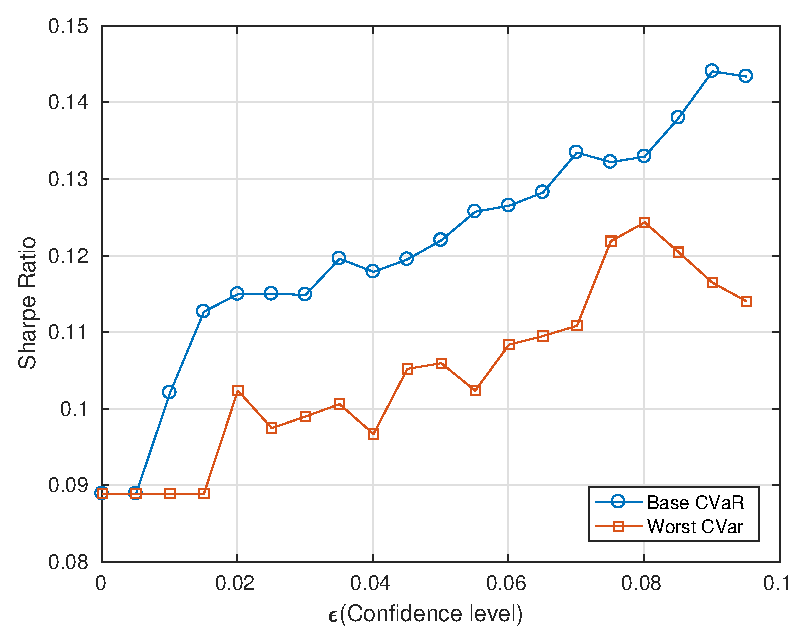
\includegraphics[height=3.825cm,width=0.35\textwidth]{CVaR/bse100_market/sr_cvar_3.eps}

   \caption{Sharpe ratio plot for CVaR and WCVaR in case of Market Data for $l=3$}
   \label{fig:6.4}
\end{figure}

\begin{block}{Common observation inferred from three cases}
WCVaR model performs superior as compared to the CVaR model in the case of simulated data and vice-versa in the case of market data.
\end{block}

\end{frame}

\section{Relevant Insights}

\begin{frame}{Relevant Insights}{Robust Optimization in Mean-Variance Analysis}
\begin{table}[!h]
    \centering
    \small
    \captionsetup{justification=centering}
   %\begin{tabular}{||p{6cm}|p{3cm}|p{3cm}||}
   \begin{tabular}{||c|c|c||}
   \hline
  & \#stocks = 31 & \#stocks = 98 \\
  \hline
 \#generated\textunderscore simulations = 1000  & 0.2    &0.244\\
 \#generated\textunderscore simulations = $\zeta$ & 0.218  & 0.233 \\
 Market data & 0.2 & 0.194 \\
 \hline
\end{tabular}
    \caption{\centering{The maximum average Sharpe ratio compared by varying the number of stocks in different kinds of scenarios.}}
    \label{tab:no_stocks}
\end{table}
\begin{block}{From the Standpoint of Number of Stocks}
More the number of stocks, more is the diversification of the portfolio. This is the principle behind this type of observation. However, in market data, the Sharpe ratio in case of more number of stocks is less than that of the case with smaller number of stocks. We believe that this kind of behaviour is due to relatively low amount of data available for higher number of stocks.
\end{block}
\vfill
\end{frame}

\begin{frame}{Relevant Insights}{Robust Optimization in Mean-Variance Analysis}

\begin{table}[!h]
    \centering
    \small
    \captionsetup{justification=centering}
   %\begin{tabular}{||p{4cm}|p{4cm}|p{4cm}||}
   \begin{tabular}{||c|c|c||}
   \hline
  & \#samples = 1000 & \#samples = $\zeta$ \\
  \hline
  \#stocks = 31  & 0.2    &0.218\\
 \#stocks = 98 &   0.244  & 0.233 \\
 \hline
\end{tabular}
    \caption{The maximum average Sharpe ratio compared by varying the number of stocks in different kinds of scenarios.}
    \label{tab:no_samples}
\end{table}
\begin{block}{From the Standpoint of Number of Simulations}
We explain this type of behaviour as follows: In the available real market data, the number of instances available for larger number of stocks is relatively low. So, when  more number of samples were generated, we observe higher Sharpe ratios when compared to $\zeta$ number of simulations. We are yet to explore the reason behind such type of behaviour when smaller number of stocks are considered.
\end{block}
\vfill
\end{frame}

\begin{frame}{Relevant Insights}{Robust Optimization in Mean-Variance Analysis}
\begin{table}[!h]
    \centering
    \small
    \captionsetup{justification=centering}
   %\begin{tabular}{||p{4cm}|p{4cm}|p{4cm}||}
   \begin{tabular}{||c|c|c||}
   \hline
  & Simulated data & Real Market data \\
  \hline
  \#stocks = 31  & 0.218    &0.2\\
 \#stocks = 98 &   0.244  & 0.194  \\
 \hline
\end{tabular}
    \caption{The maximum average Sharpe ratio compared by varying the type of the data in different kinds of scenarios.}
    \label{tab:data_type}
\end{table}
\begin{block}{From the Standpoint of Type of the Data}
Here the behaviour is straight forward. In both the cases, the performance in the case of simulated data is better than the real market data. This is clear from the fact that the real market data are difficult to model and hardly may follow any distribution, whereas the simulated data simply follows multivariate normal distribution with mean and covariances as the true values obtained from the data.
\end{block}
\vfill
\end{frame}

\begin{frame}{Relevant Insights}{Robust Optimization in VaR Minimization}
\begin{table}[!h]
  \centering
  \tiny
    \captionsetup{justification=centering}
  %\begin{tabular}{|l|l|l|l|l|l|l|}
  \begin{tabular}{|c|c|c|c|c|c|c|}
    \hline
   \multirow{2}{*}{} $N$ &
      \multicolumn{3}{c|}{$N=31$} &
      \multicolumn{3}{c|}{$N=98$}  \\
    \hline
    Type of & Market & Sim. data & Sim. data & Market & Sim. data & Sim. data \\
    data & data & $\zeta$ samples & $1000$ samples & data & $\zeta$ samples & $1000$ samples \\
    \hline
    VaR & 0.111 & 0.0884 & 0.0987 & 0.119 & 0.0674 & 0.137 \\
    \hline
    WVaR & 0.0998 & 0.0765 & 0.0989 & 0.124 & 0.103 & 0.16 \\
    \hline
    
  \end{tabular}
  \caption{Comparison of the average Sharpe ratio for the VaR and WVaR models in various scenarios.}
  \label{tab:var_conc}
\end{table}
\begin{block}{From the Standpoint of the number of stocks}
We observe that the WVaR model exhibits superior performance than the Base VaR model in case of larger number of stocks irrespective of the type of the data. We attribute this type of pattern to the following reasons: The errors in the estimation of moments' pair of the asset returns accumulates as the number of stocks increases which leads to high data uncertainty. The Worst-case robust model can handle the data uncertainty in a better way than the Base VaR model.
\end{block}
\end{frame}

\begin{frame}{Relevant Insights}{Robust Optimization in VaR Minimization}

\begin{block}{From the Standpoint of the number of simulations}
 For the case $N=98$, the better performance of WVaR model is attributed to the reason above. But when $N=31$, the performance of the optimal portfolio, in case of 1000 samples is more than that of the case involving $\zeta$ number of simulations. The reason can be attributed to the subroutine of the Non Parametric Bootstrap Algorithm, that uses sampling with replacement. Hence, more the number of  samples, better are the bounds which leads to the improvement in the performance of the portfolio.
\end{block}
\end{frame}
\begin{frame}{Relevant Insights}{Robust Optimization in VaR Minimization}
\begin{block}{From the Standpoint of the type of the data}
When $N=31$, the equivalent performance of the WVaR model with Base VaR model in case of simulated data can be attributed to the following reason: The real market data is difficult to model and may not follow any distribution, whereas the simulated data follows the multivariate normal distribution. The reason for the out-performance of WVaR model over the Base VaR model when $N=98$ stocks are considered is discussed in the above slides.
\end{block}
\end{frame}
\begin{frame}{Relevant Insights}{Robust Optimization in CVaR Minimization}
\begin{table}[!h]
  \centering
  \tiny
    \captionsetup{justification=centering}
  %\begin{tabular}{|l|l|l|l|l|l|l|}
  \begin{tabular}{|c|c|c|c|c|c|c|}
    \hline
   \multirow{2}{*}{} $N$ &
      \multicolumn{3}{c|}{$N=31$} &
      \multicolumn{3}{c|}{$N=98$}  \\
    \hline
    Type of & Market & Sim. data & Sim. data & Market & Sim. data & Sim. data \\
    data & data & $\zeta$ samples & $1000$ samples & data & $\zeta$ samples & $1000$ samples \\
    \hline
    CVaR & 0.0856 & 0.103 & 0.0929 & 0.121 & 0.0963 & 0.156 \\
    \hline
    WCVaR & 0.0611 & 0.106 & 0.0969 & 0.105 & 0.102 & 0.165 \\
    \hline
  \end{tabular}
  \caption{Comparison of the average Sharpe ratio for the CVaR and WCVaR models.}
  \label{tab:cvar_conc}
\end{table}

\begin{block}{From the Standpoint of Number of Stocks}
For Market Data, CVaR performs better than WCVaR regardless of no. of stocks. This is because of lack of knowledge about the return distribution in market data. For Simulated Data with $1000$ samples, uptrend observed in the performance of WCVaR vis-\`a-vis CVaR because being a robust risk measure, it diversifies over worst-case scenarios as well through mixture distribution uncertainty. For Simulated data with $\zeta$ samples, there's a decline in the performance of both models as N increases to 98 despite involving similar comparative inference. The reason isn't obvious.
    

\end{block}

\end{frame}

\begin{frame}{Relevant Insights}{Robust Optimization in CVaR Minimization}

\begin{block}{From the Standpoint of Number of Simulations}
For the case involving $\zeta$ simulations, the WCVaR model performs at par with the CVaR model irrespective of the number of stocks. Same inference can be drawn with $1000$ simulated samples as well. Hence, we note equivalent performance of the two models in each simulation study.
\end{block}

\begin{block}{From the Standpoint of Type of the Data}
Due to similar reasons as in VaR minimization, an opposite trend is observed in the case of real market data when the number of stocks is less ($N=31$). Similar observation is inferred for the market data on taking into account the larger number of stocks ($N=98$). 
\end{block}

\end{frame}


\section{Concluding Remarks}

\begin{frame}{Concluding Remarks}{Robust Optimization in Mean-Variance Analysis}

\begin{itemize}
    \item {We observe that robust optimization with ellipsoidal uncertainty set performs superior or equivalent as compared to the Markowitz model, in the case of simulated data, similar to the results reported by Santos. In addition, we observe favorable results in the case of market data as well.  }
    \item {Better performance of robust formulation having separable uncertainty set in comparison to Markowitz model is in line with the previous study on the same robust model by T{\"u}t{\"u}nc{\"u} and Koenig \cite{tut}.}
\end{itemize}
    
\end{frame}

\begin{frame}{Concluding Remarks}{Robust Optimization in VaR and CVaR minimization}
\begin{itemize}
    \item Akin to mean variance analysis, there is a problem of lack of robustness in the classical formulations of VaR and CVaR minimization.
    \item We discuss and assess the performance of the robust counterparts for these optimization problems that have been formulated to address this concern.
    \item Motivated by the results by Ghaoui et al. \cite{ghaoui03}, we formulate the worst case robust version of the VaR model using separable uncertainty set.
    \item Regardless of the type of the data, be it from real market or from a simulated environment, we observe favourable results for the worst case VaR model with Sharpe ratio as the performance measure when the portfolio comprises higher number of stocks.
\end{itemize}
   
\end{frame}

\begin{frame}{Concluding Remarks}{Robust Optimization in VaR and CVaR minimization}
\begin{itemize}
    \item{In contrast to the results reported by Zhu, we observe that the base-case CVaR performs better than the worst-case CVaR in the case of market data irrespective of the number of stocks comprising in the optimal portfolio. This could be attributed to the following two reasons:
    \begin{enumerate}
        \item Incorporation of different weight constraints in our optimization problem.
        \item Unlike Zhu, our work uses Sharpe Ratio as a performance measure.
    \end{enumerate}}
    \item{In the case of simulated data, a favourable inference is drawn by noting superior or equivalent performance of the worst case CVaR vis-\`a-vis the base case CVaR.}
\end{itemize}
\end{frame}


\begin{frame}{Papers from the B.Tech project work}
    \begin{itemize}
        \item{ [Communicated Paper] Can Robust Optimization Offer Improved Portfolio Performance?: An Empirical study of Indian Market. International Journal of Finance and Economics (IJFE), Wiley.}
        \item{ [In Preparation] Can Robust Risk Minimization Offer Improved Portfolio Performance?: A Perspective from the Indian Market.}
        
    \end{itemize}
\end{frame}





%------------------------------------------------



%------------------------------------------------
%\section{Second Section}
%------------------------------------------------



%------------------------------------------------



%------------------------------------------------





% \begin{frame}[fragile] % Need to use the fragile option when verbatim is used in the slide
% \frametitle{Citation}
% An example of the \verb|\cite| command to cite within the presentation:\\~

% This statement requires citation \cite{p1}.
% \end{frame}

%------------------------------------------------
\section{References}

\begin{frame}
\frametitle{References}
\footnotesize{
\begin{thebibliography}{99} % Beamer does not support BibTeX so references must be inserted manually as below
% \bibitem[Smith, 2012]{p1} John Smith (2012)
% \newblock Title of the publication
% \newblock \emph{Journal Name} 12(3), 45 -- 678.
\bibitem{mark1} H. M. Markowitz. Portfolio selection. The journal of finance, 7(1):77–91,
1952.
\bibitem{michaud} R. O. Michaud. The markowitz optimization enigma: Is ’optimized’ optimal? Financial Analysts Journal, 45(1):31–42, 1989.
\bibitem{broadie} M. Broadie. Computing efficient frontiers using estimated parameters. Annals of Operations Research, 45(1):21–58, Dec 1993.
\bibitem{black} F. Black and R. Litterman. Global portfolio optimization. Financial Analysts Journal, 48(5):28–43, 1992.
\bibitem{tut} R. H. T{\"u}t{\"u}nc{\"u} and M. Koenig. Robust asset allocation. Annals of Operations Research, 132(1-4):157–187, 2004.
% \bibitem{scherer} B. Scherer. Can robust portfolio optimisation help to build better portfolios? Journal of Asset Management, 7(6):374–387, Mar 2007.
\bibitem{santos} A. Santos. The Out-of-Sample Performance of Robust Portfolio Optimization. Brazilian Review of Finance, 8(2):141--166, 2010.

\bibitem{fabozzi} F. J. Fabozzi, P. N. Kolm, D. Pachamanova, and S. M. Focardi. Robust Portfolio Optimization and Management. Wiley, 2007.
\end{thebibliography}
}
\end{frame}

\begin{frame}
\frametitle{References}
\footnotesize{
\begin{thebibliography}{99} % Beamer does not support BibTeX so references must be inserted manually as below
% \bibitem[Smith, 2012]{p1} John Smith (2012)
% \newblock Title of the publication
% \newblock \emph{Journal Name} 12(3), 45 -- 678.
\bibitem{ghaoui03} Ghaoui, L. E. Ghaoui, M. Oks, and F. Oustry. Worst-case value-at-risk and ro-
bust portfolio optimization: A conic programming approach. Operations Research, 51(4):543–556, 2003.
\bibitem{ju98} X. Ju and N. D. Pearson. Using value-at-risk to control risk taking: how wrong can you be? OFOR Working Paper Series, no. 98-08, 1998
\bibitem{bertsimas05} D. Bertsimas and I. Popescu. Optimal inequalities in probability theory: A convex optimization approach. SIAM Journal on Optimization, 15(3):780–804, 2005.
\bibitem{rockafellar1} R. T. Rockafellar and S. Uryasev. Optimization of conditional value-at-risk. Journal of risk, 2:21-42, 2000.
\bibitem{rockafellar2} R. T. Rockafellar and S. Uryasev. Conditional value-at-risk for general loss distributions. Journal of Banking \& Finance, 26(7):1443--1471, 2002.
\bibitem{artzner} P. Artzner, F. Delbaen, J. Eber and D. Heath. Coherent measures of risk. Mathematical Finance, 9(3):203--228, 1999.
\bibitem{zhu} S. Zhu and M. Fukushima. Worst-case conditional value-at-risk with application to robust portfolio management. Operations Research, 57(5):1155--1168, 2009.

\end{thebibliography}
}
\end{frame}

%------------------------------------------------

\begin{frame}
\Huge{\centerline{The End}}
\end{frame}

%----------------------------------------------------------------------------------------

\end{document}